\documentclass[11pt]{article}
\title{Winberry 2018 Code Replication}
\author{Brandon Kaplowitz \thanks{Immense thanks to Tom Winberry for writing the original 2018 code which my code is heavily adopted from and the many helpful comments in understanding it.}}
\usepackage{todonotes}

\usepackage{amsmath}
\usepackage[authordate,backend=biber]{biblatex-chicago}
\usepackage{mathtools}
\usepackage{graphicx}
\usepackage{caption}
\usepackage{hyperref}
\usepackage{subcaption}
\usepackage{float}
\usepackage{xcolor,amsmath}
\usepackage[linesnumbered,ruled,vlined]{algorithm2e}
\addbibresource{replication_sources.bib}

\newcommand{\code}[1]{\texttt{#1}}
\DontPrintSemicolon

% Define pseudocode formatting
\renewcommand{\KwSty}[1]{\textnormal{\textcolor{blue!90!black}{\ttfamily\bfseries #1}}\unskip}
\renewcommand{\ArgSty}[1]{\textnormal{\ttfamily #1}\unskip}
\SetKwComment{Comment}{\color{green!50!black}// }{}
\renewcommand{\CommentSty}[1]{\textnormal{\ttfamily\color{green!50!black}#1}\unskip}
\newcommand{\assign}{\leftarrow}
\newcommand{\var}{\texttt}
\newcommand{\FuncCall}[2]{\texttt{\bfseries #1(#2)}}
\SetKwProg{Function}{function}{}{}
\renewcommand{\ProgSty}[1]{\texttt{\bfseries #1}}

\begin{document}
\maketitle
\section{Introduction}
This document walks through the main approaches used in replicating \cite{Winberry2018} and the current limitations/future extensions possible. The code is written almost entirely in Python, except for the perturbation component which is written using Dynare in contrast to the original code which was done purely in Matlab/Dynare. Thanks must be given to both Tom Winberry for the original code and the Dynare code library. The Python code uses several key packages including:
\begin{itemize}
\item Numpy 
\item Scipy
\item Icecream (for debugging)
\item Logging (for debugging)
\item Base.IO
\item Base.Time
\item Matplotlib
\item Numba (for speeding up portions)	
\end{itemize}
and the code would not be possible without these libraries.

\section{Algorithms (Stationary)}
Now I will give a brief description of the key aspects of the code in a verbal Pseudocode format (for succinctness). 
First, we go through and set the key parameters of the model and approximation in the \code{replication\_winberry\_2018.ipynb} main file.
Then we run \code{create\_grids.py}, which respectively construct the grids we need on the asset, and epsilon space, as well as scaled versions of the asset space between 0 and 1 to find the Chebyshev zeros. We then run \code{create\_polynomials.py} which generates the Chebyshev polynomials over the asset space which we use to interpolate. 
Now, we get to the first of our three main algorithms, Young's 2010 method to find a histogram approximation to the steady state endogenous distribution and an estimate of steady state capital. It is implemented in
 \code{compute\_MC\_Residual\_Histogram.py} with details left to the appendix of this Description.  Next we run \code{compute\_MC\_Residual\_poly.py} to compute the estimated parametric (exponential) form of the SS distribution and a new guess of $K_{SS}$. Again high-level descriptions of the implementation are moved to the appendix. 
Finally, we graph our extract policy functions for savings and consumption for employed $\epsilon =1$ and unemployed $\epsilon =0$ individuals as seen in figures \ref{con_sav_rep} and \ref{con_sav_orig}. We also plot the endogenous distribution of asset holdings in steady state using our parametric form  and Young's histogram method on our grid. We can see these exactly match the original output from Winberry (see Appendix for Graphs: \ref{dist_rep} and \ref{dist_orig})
\begin{figure*}[htp]
\begin{subfigure}{.5\textwidth}
\centering
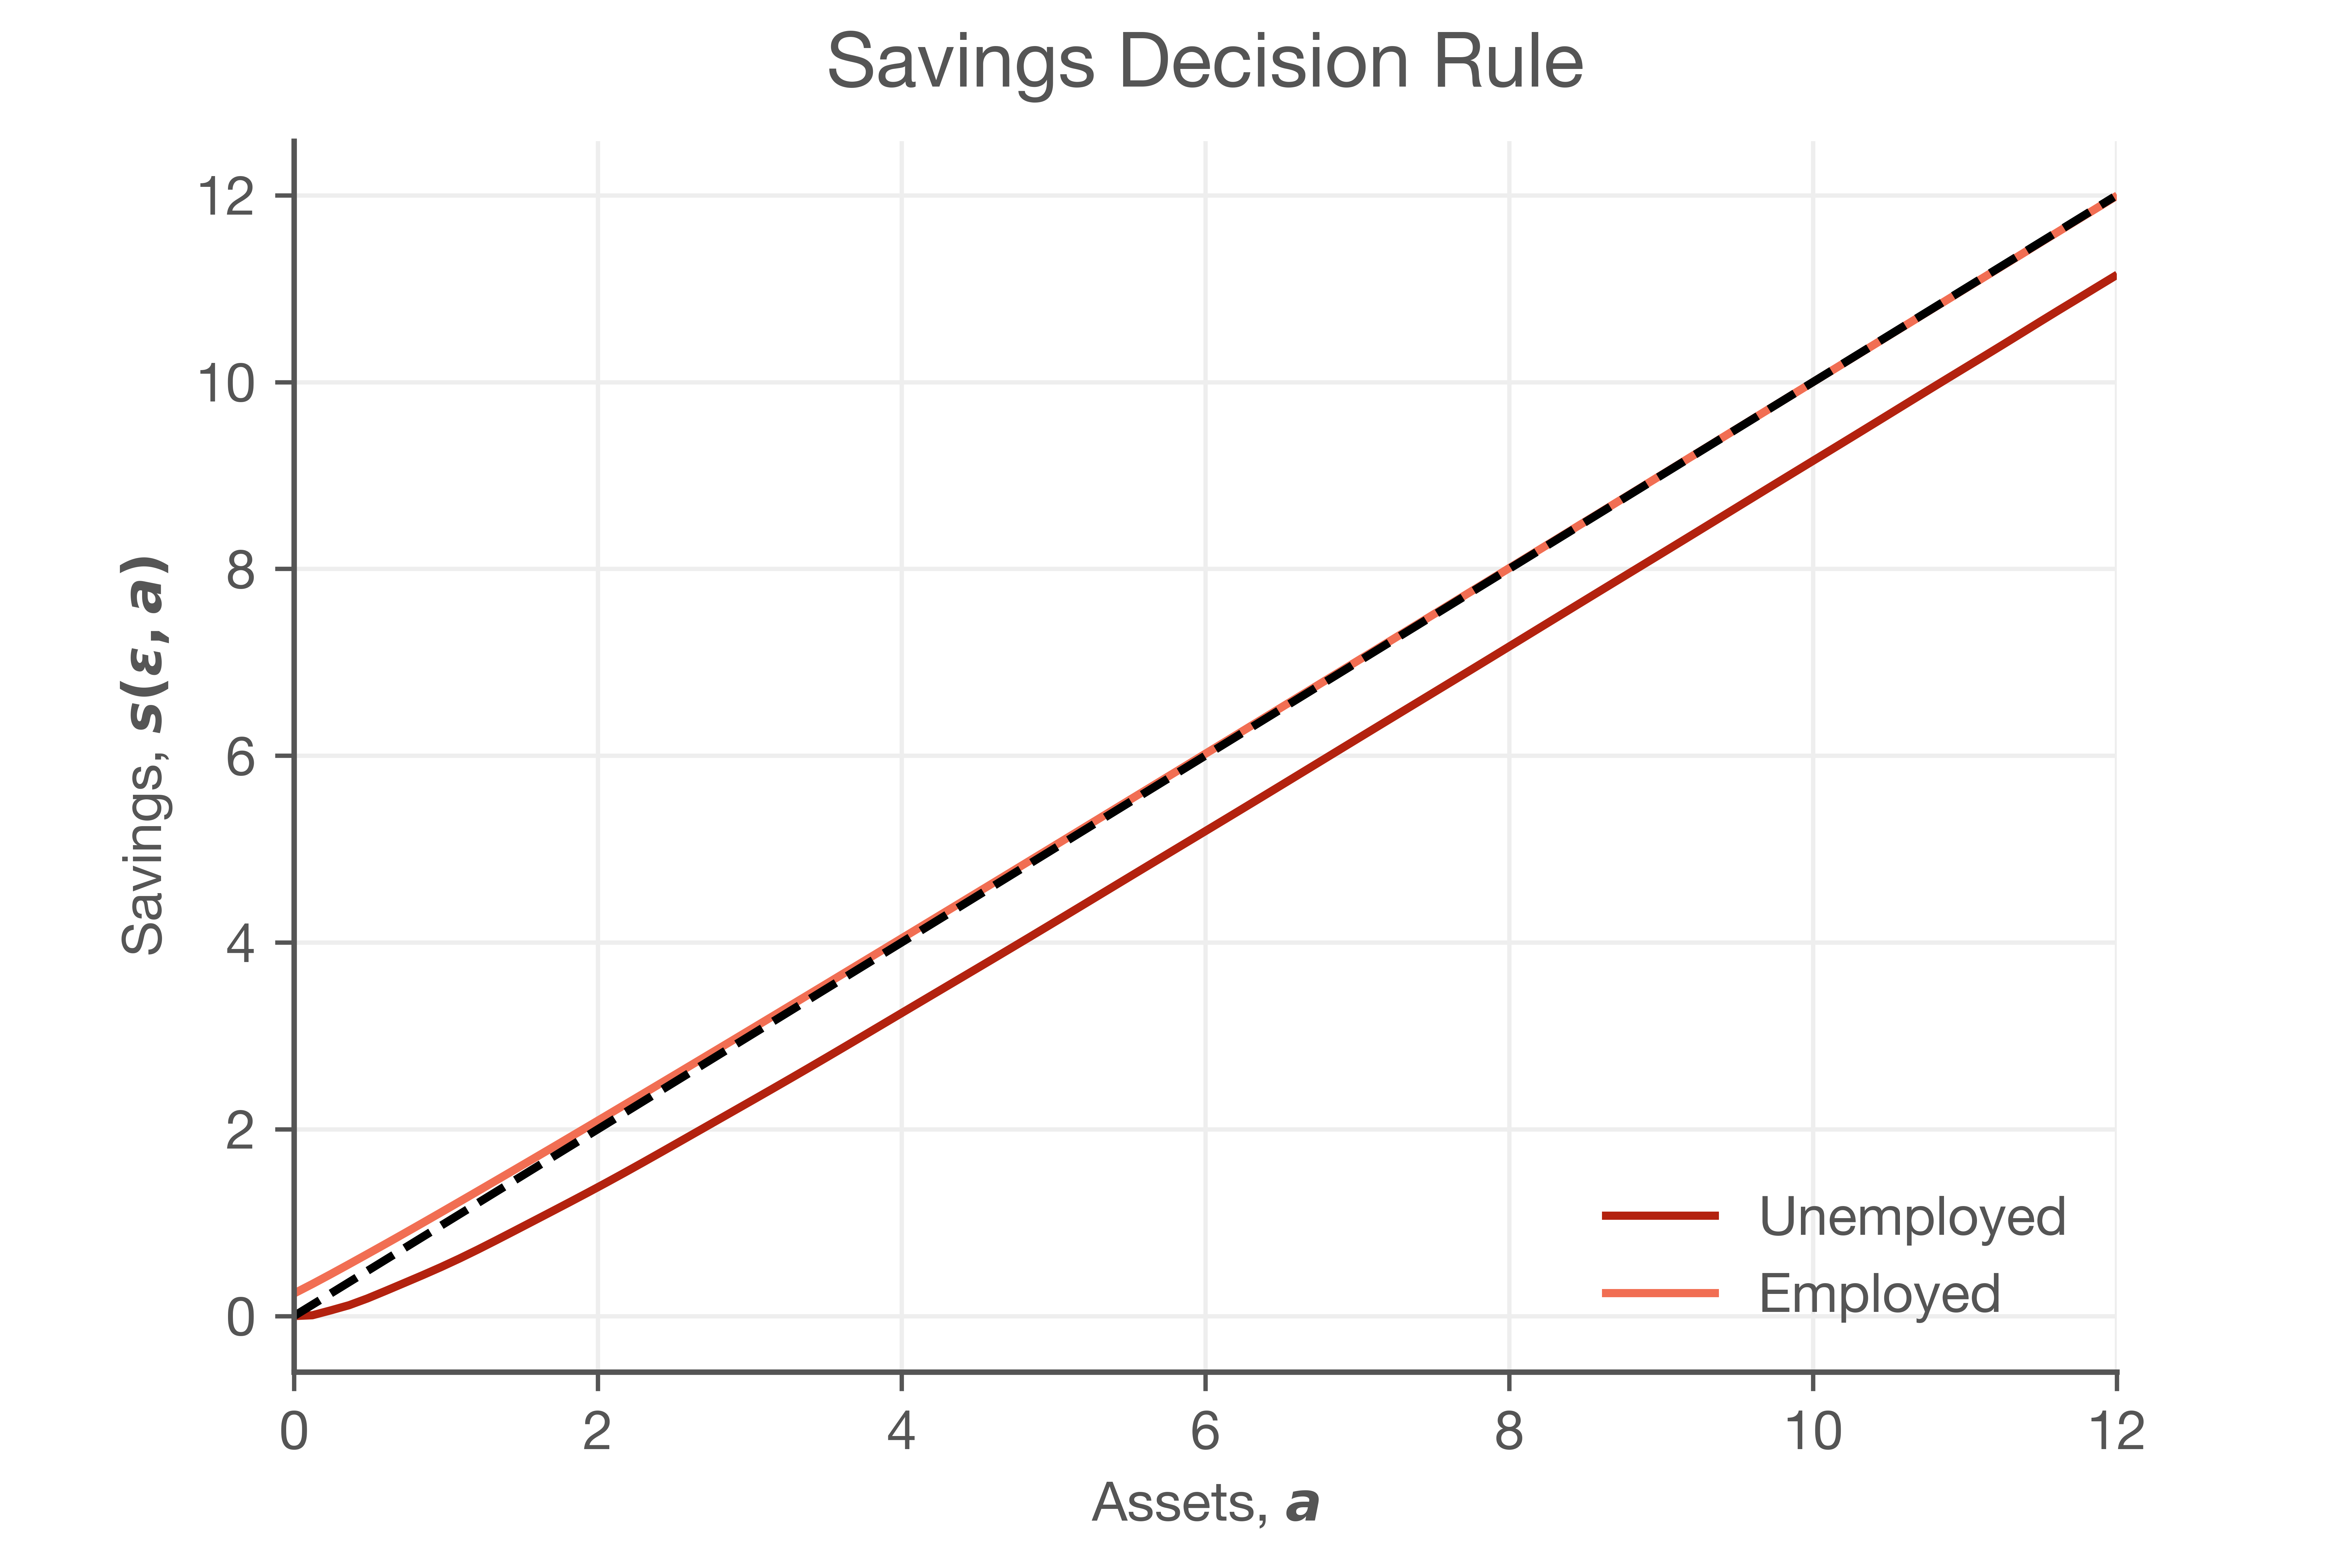
\includegraphics[scale=.45]{Figures/save_rule.png}

\end{subfigure}
\begin{subfigure}{.5\textwidth}
\centering
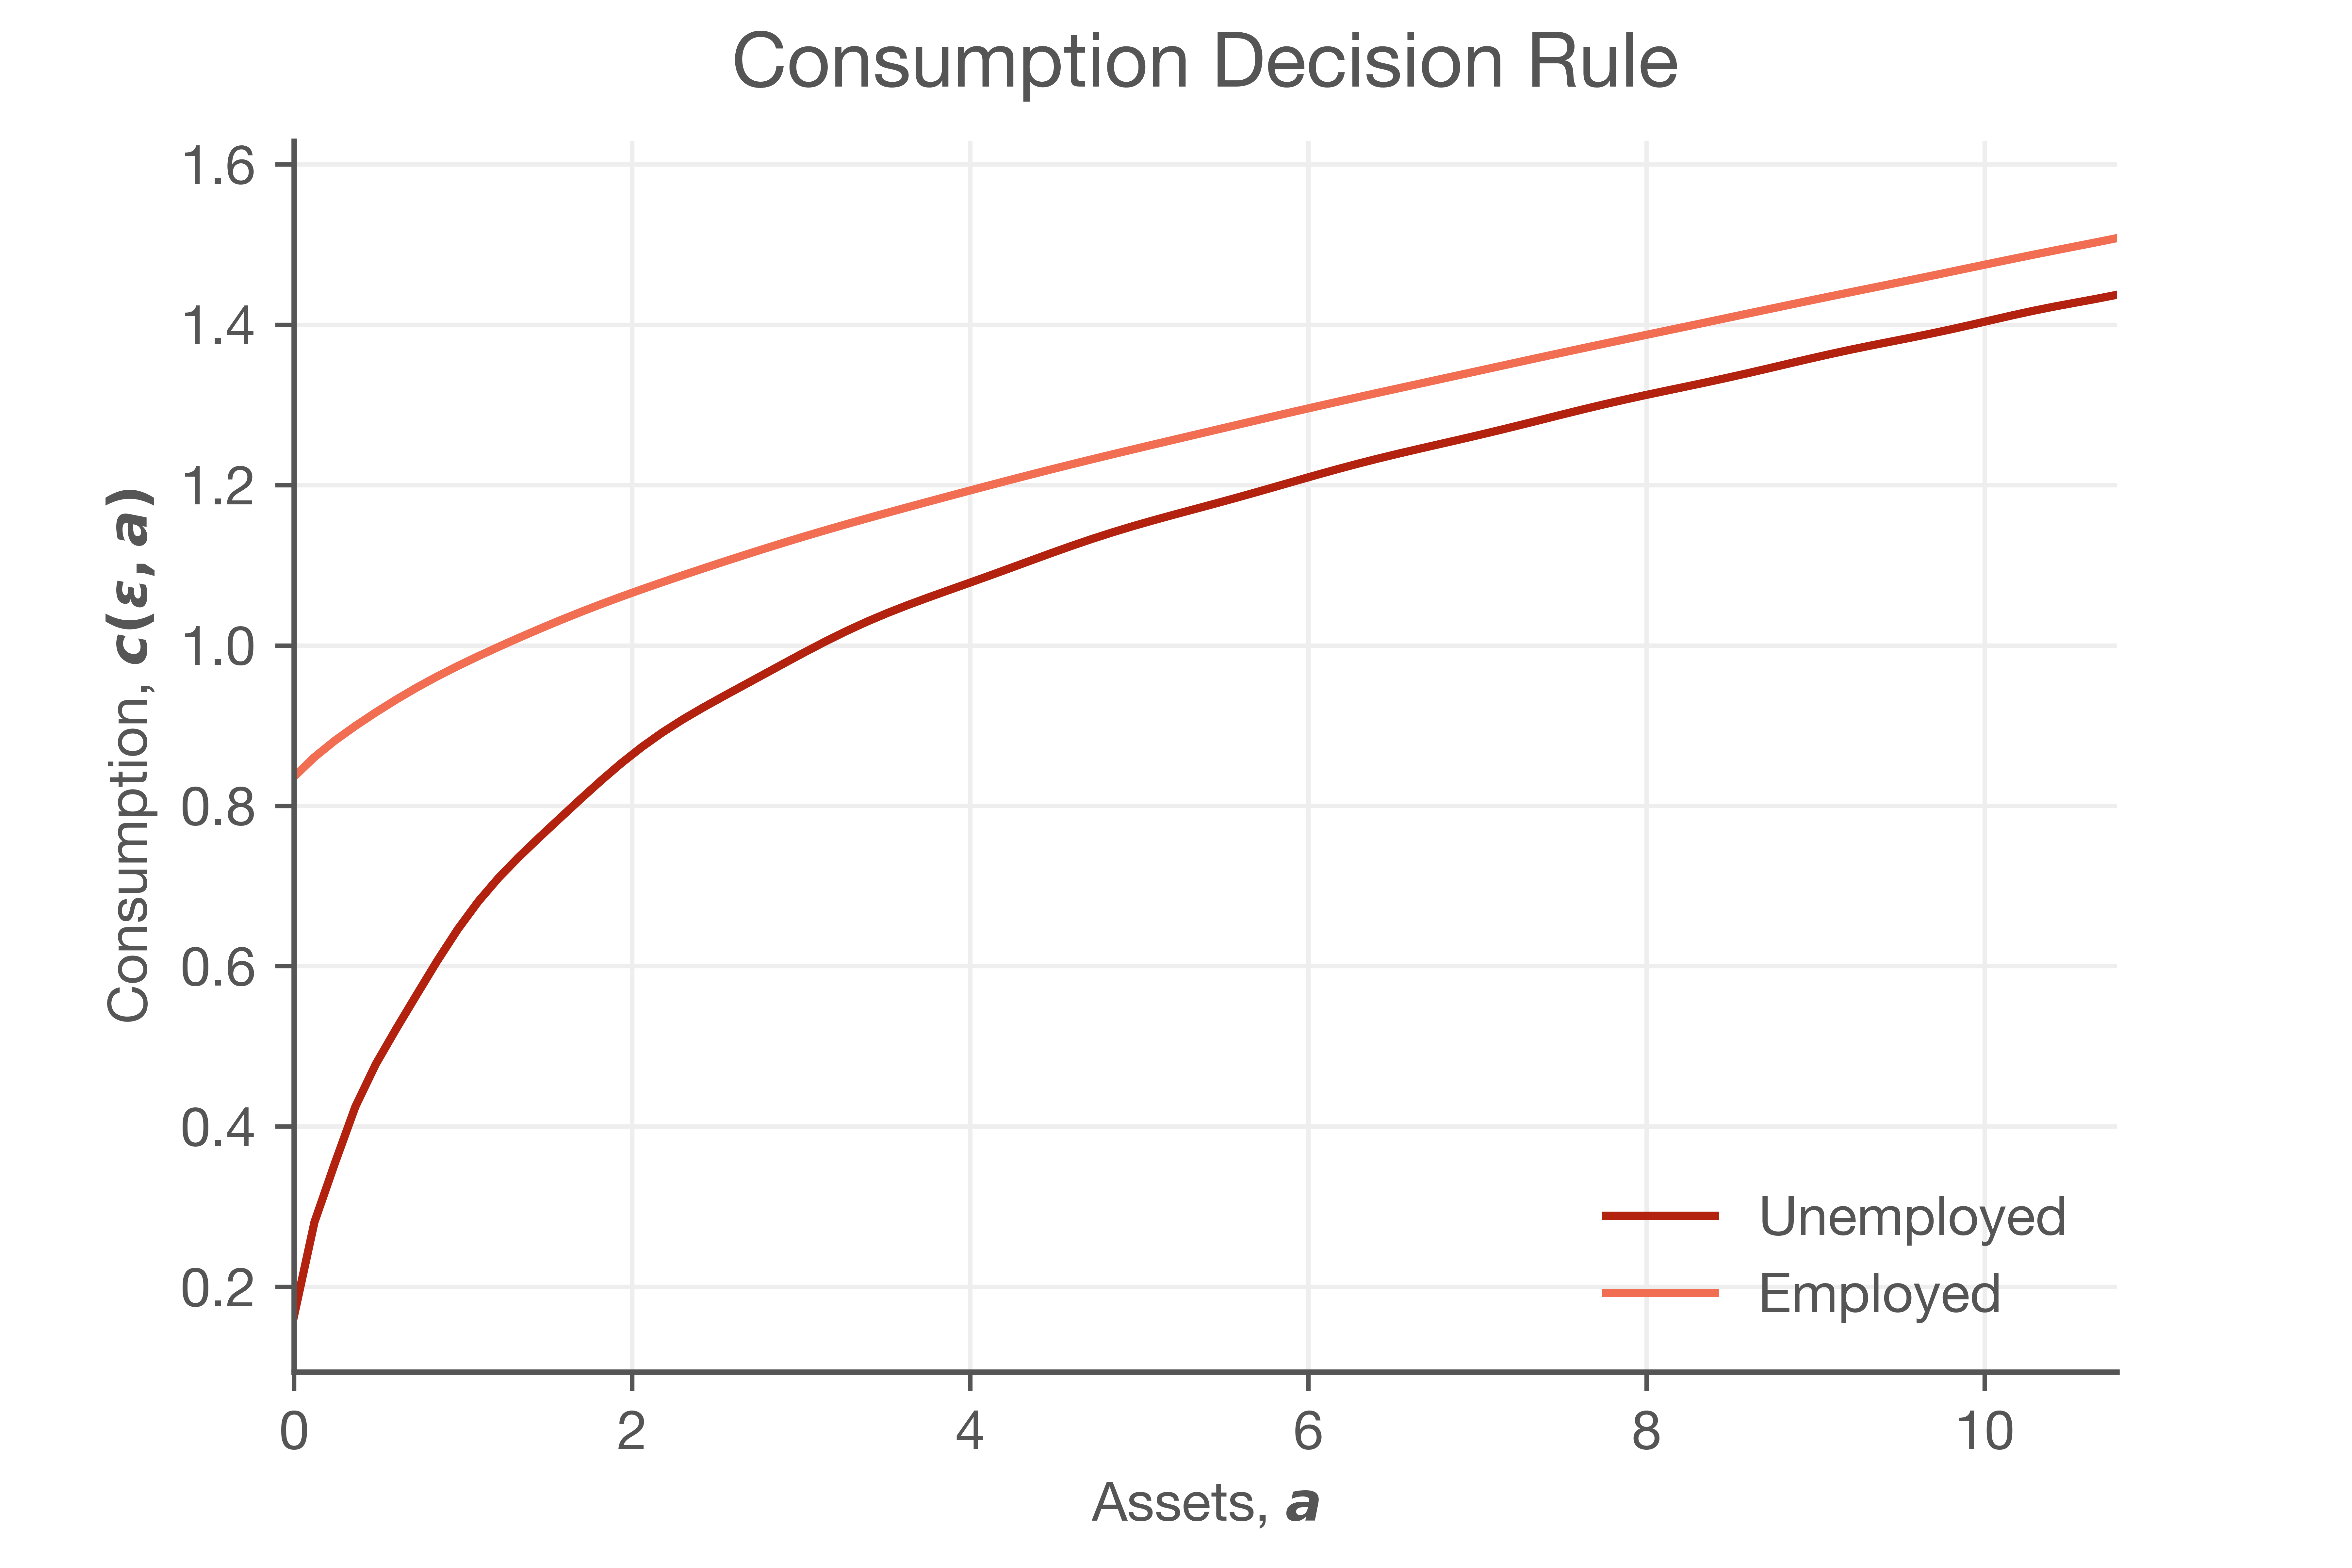
\includegraphics[scale=.45]{Figures/cons_rule.png}
\end{subfigure}
\caption{Replicated savings and consumption rules for employed and unemployed workers. Can be reproduced by running IPython notebook (.ipynb) file  }
\label{con_sav_rep}
\vspace*{\floatsep}
\centering
\includegraphics[scale=.9]{../../../../../../Desktop/Screen Shot 2021-01-25 at 1.18.01 PM}
\caption{Winberry's 2018 calculations of the implied policy rules for savings and consumption in the Aiyagari model, taken from his 2018 paper and User Guide from his website.}
\label{con_sav_orig}
\end{figure*}	


\begin{figure*}[htp]
\begin{subfigure}{.5\textwidth}
\centering
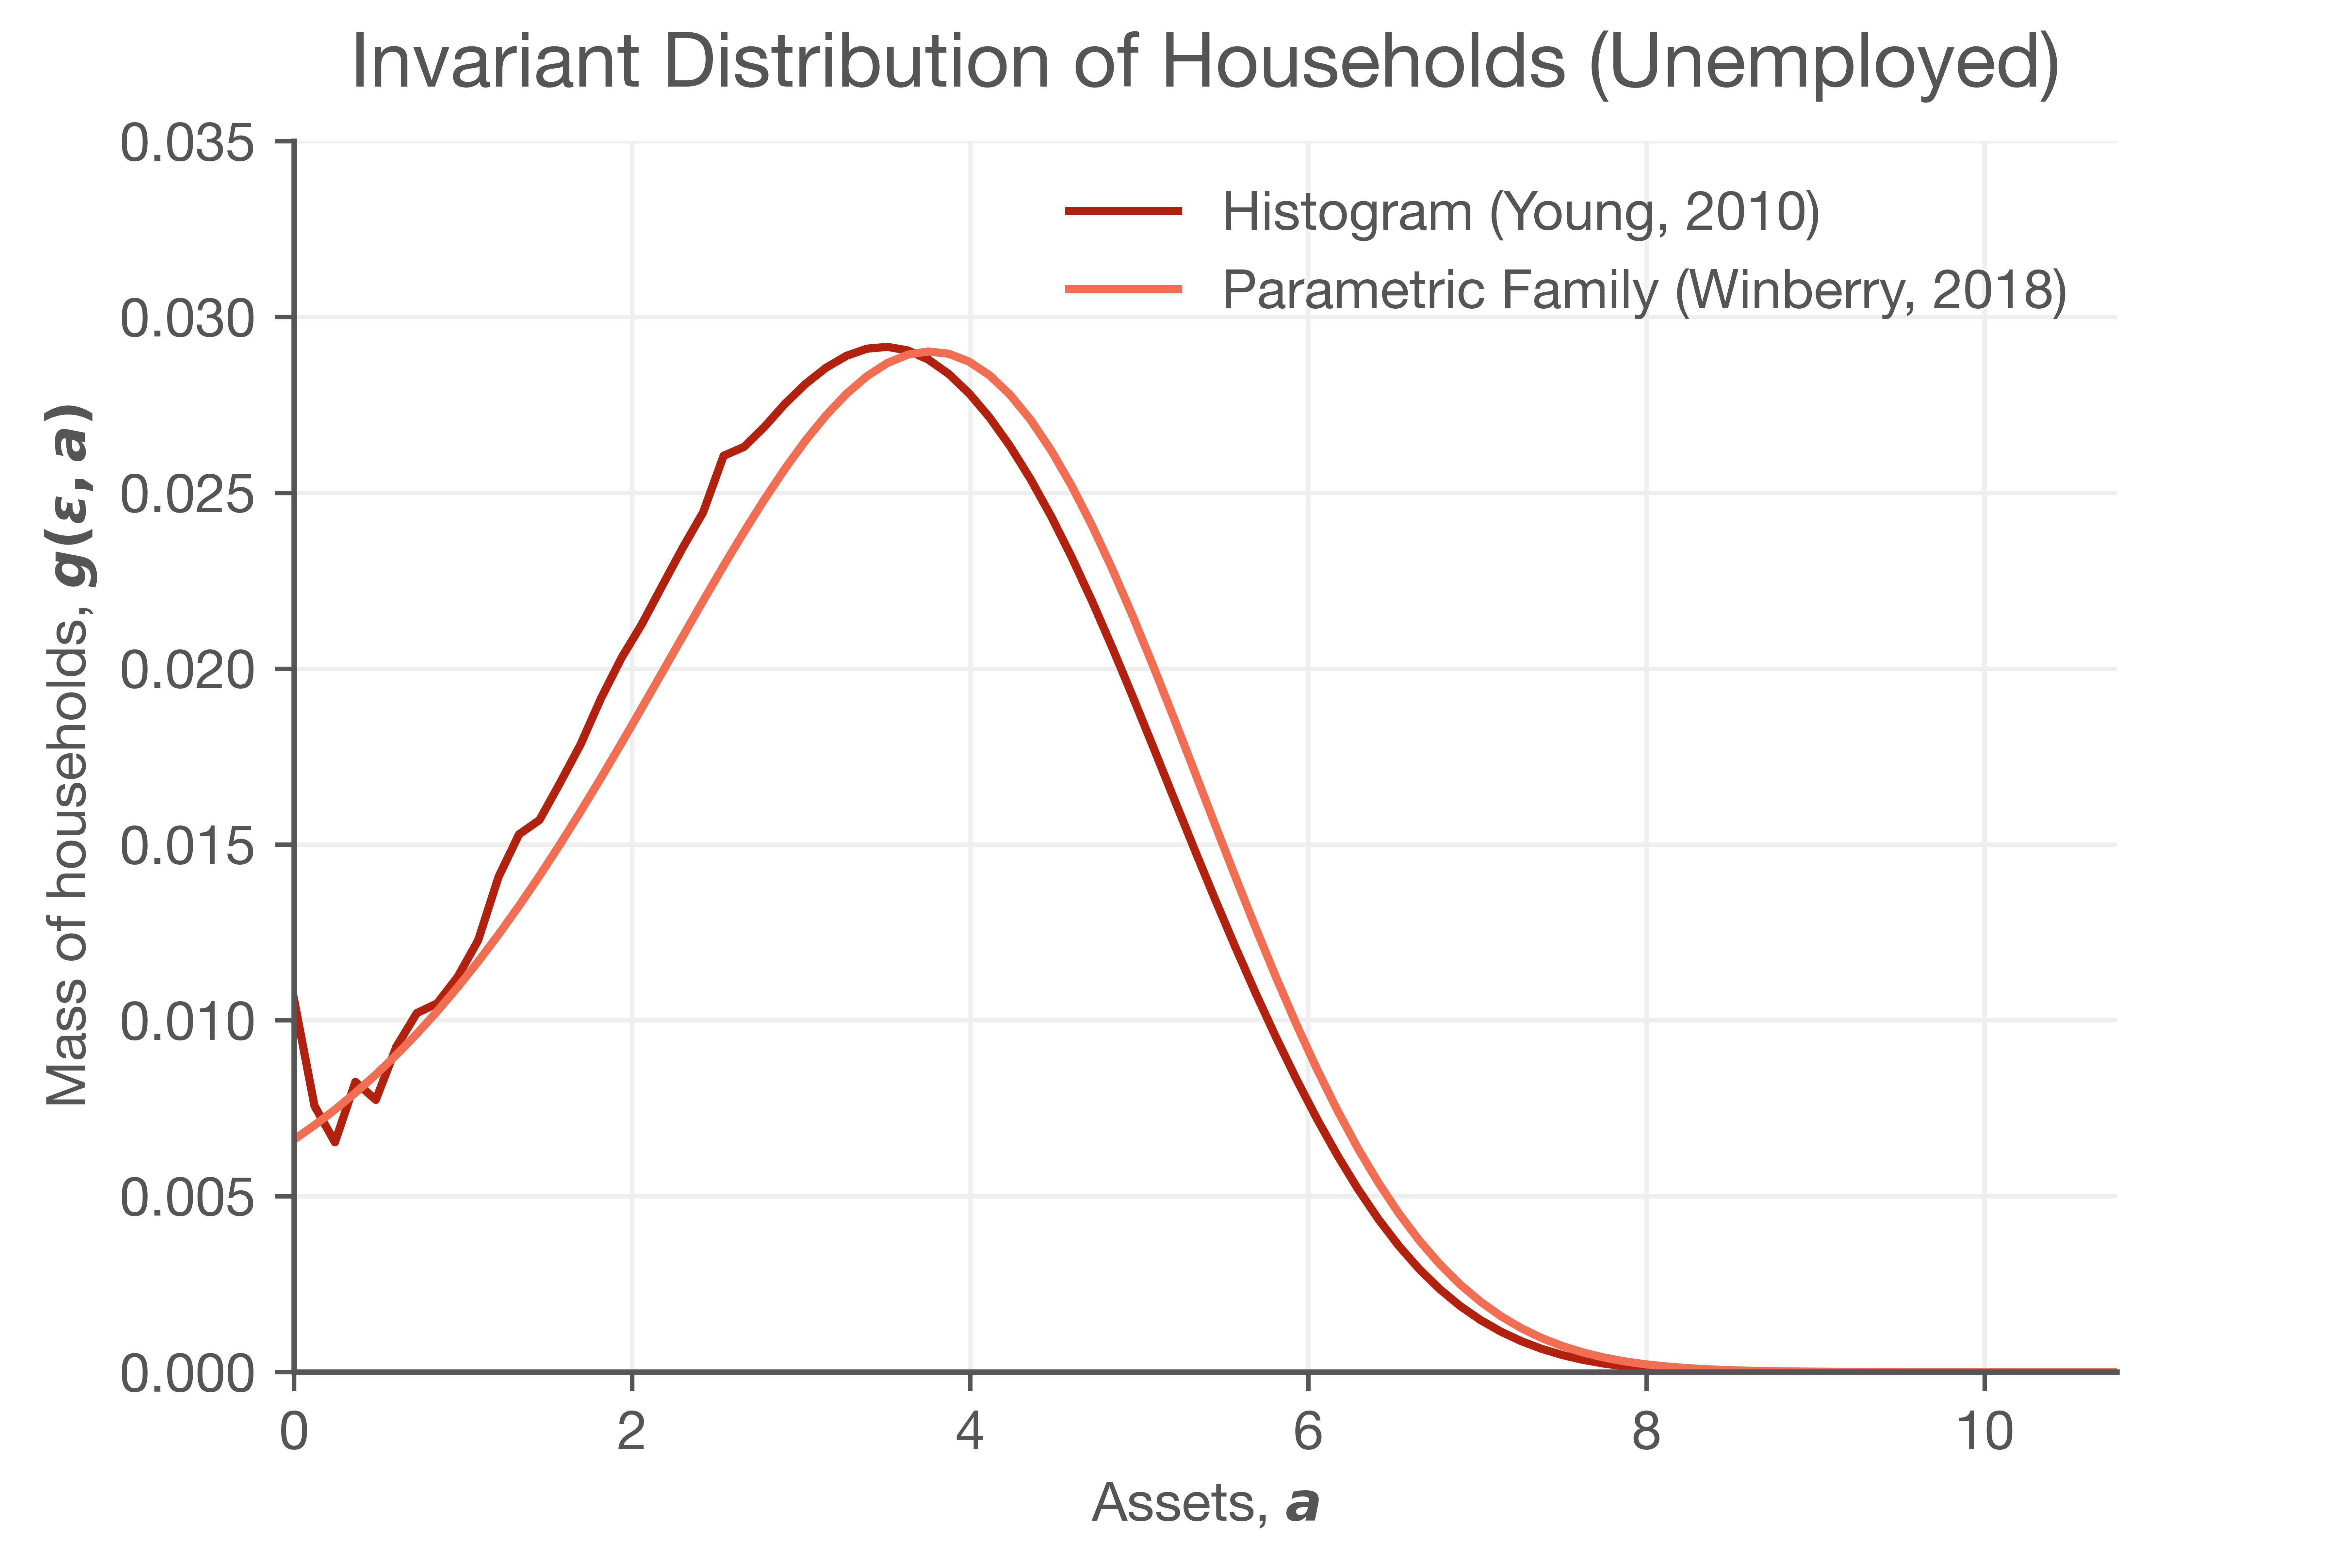
\includegraphics[scale=.45]{Figures/ivar_dist_unemployed.png}
\end{subfigure}
\begin{subfigure}{.5\textwidth}
\centering
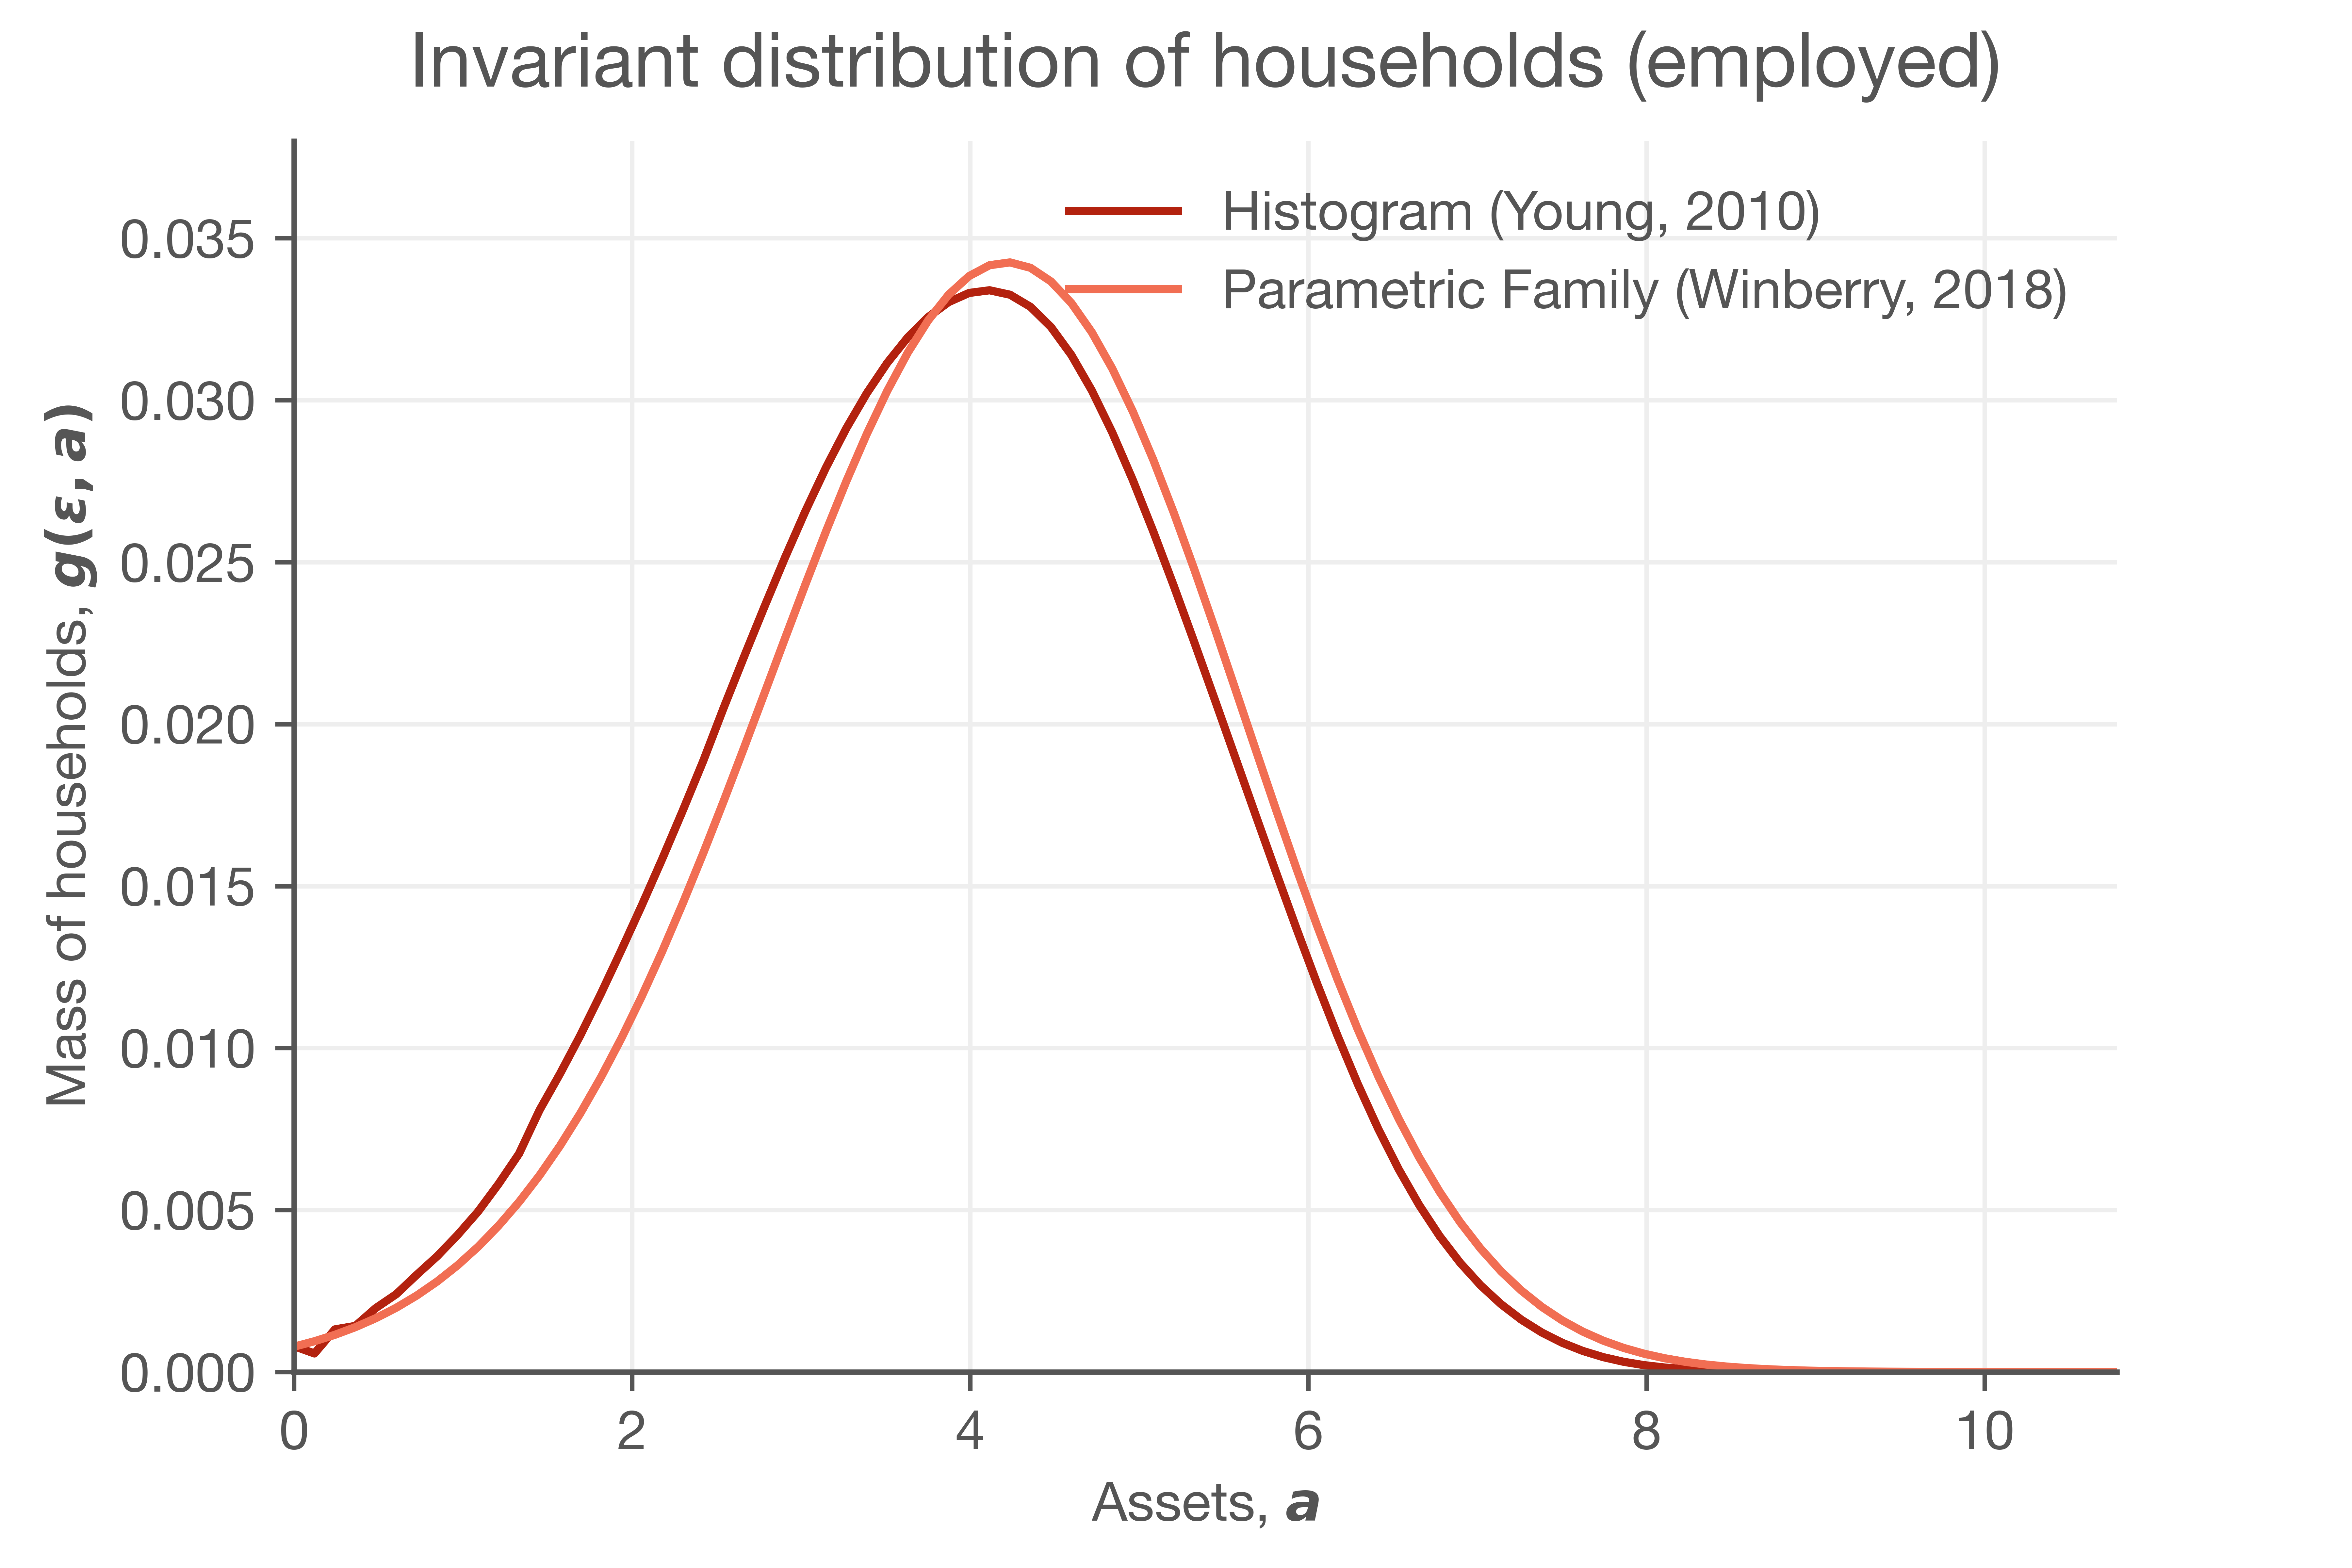
\includegraphics[scale=.45]{Figures/ivar_dist_employed.png}
\end{subfigure}
\caption{Replicated value for invariant distribution of unemployed and employed households}
\label{dist_rep}
 \vspace*{\floatsep}
\centering
\includegraphics{../../../../../../Desktop/Screen Shot 2021-01-25 at 1.26.01 PM}
\caption{Winberry's 2018 calculations of the Young 2010 method implied endogenous distribution over assets and his endogenous distribution over assets in the Aiyagari model taken from his 2018 paper and User Guide from his website.}
\label{dist_orig}
\end{figure*}	
 \section{Algorithms (Dynamics)} 
In the final portion we prepare our code to be loaded into Dynare as \code{.mat} data files. The Dynare program is executed through a series of custom \code{.mod} data files that describe the equations executed in the stationary component and then performs first (or higher order) perturbations. The Dynare file is written to and run using the Matlab package for Python that enables execution of Matlab code from within Python and so it is also executed in the IPython notebook. The \code{*\_steadystate.mod} file loads the steady state values computed from our previous code to Dynare to use as the point around which the perturbation will occur.
Due to the lack of novelty here, detailed descriptions of the .mod files are omitted, although they go through and repeat much of the procedure described around the steady state, just in terms of Dynare variables and parameters to define the relevant equations for perturbation. The perturbation method itself is a direct implementation of \cite{Schmitt-Grohe2004}. 
We can see again, that we exactly match the first order approximation result he gets graphically, and the numerical output from Dynare confirms this as seen in  figures \ref{IRF_rep} and \ref{IRF_orig}. Finally, we note that as expected, in the Aiyagari model the difference between first and higher order perturbations is negligible. 
\begin{figure*}[htp]
\begin{subfigure}{.5\textwidth}
\centering	
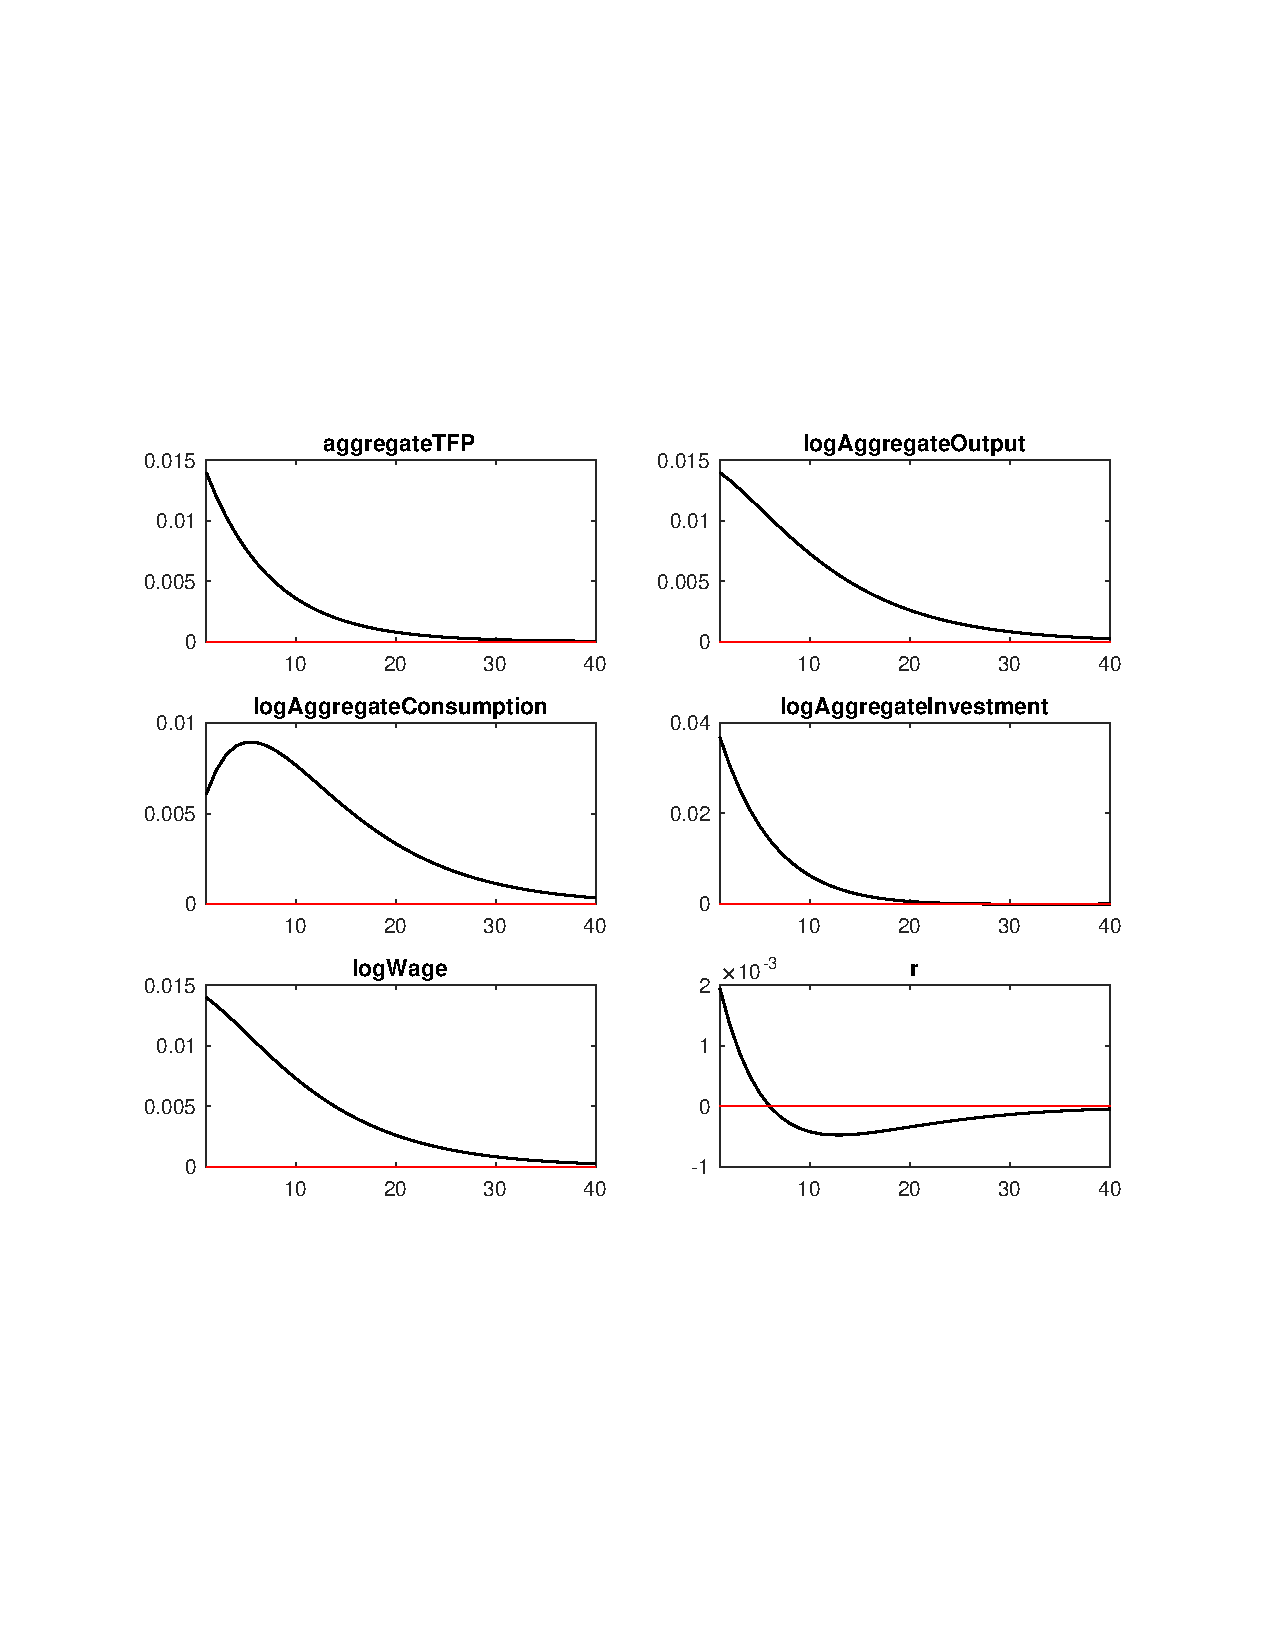
\includegraphics[scale=.33]{./order 1.pdf}
\end{subfigure}
\begin{subfigure}{.5\textwidth}
\centering
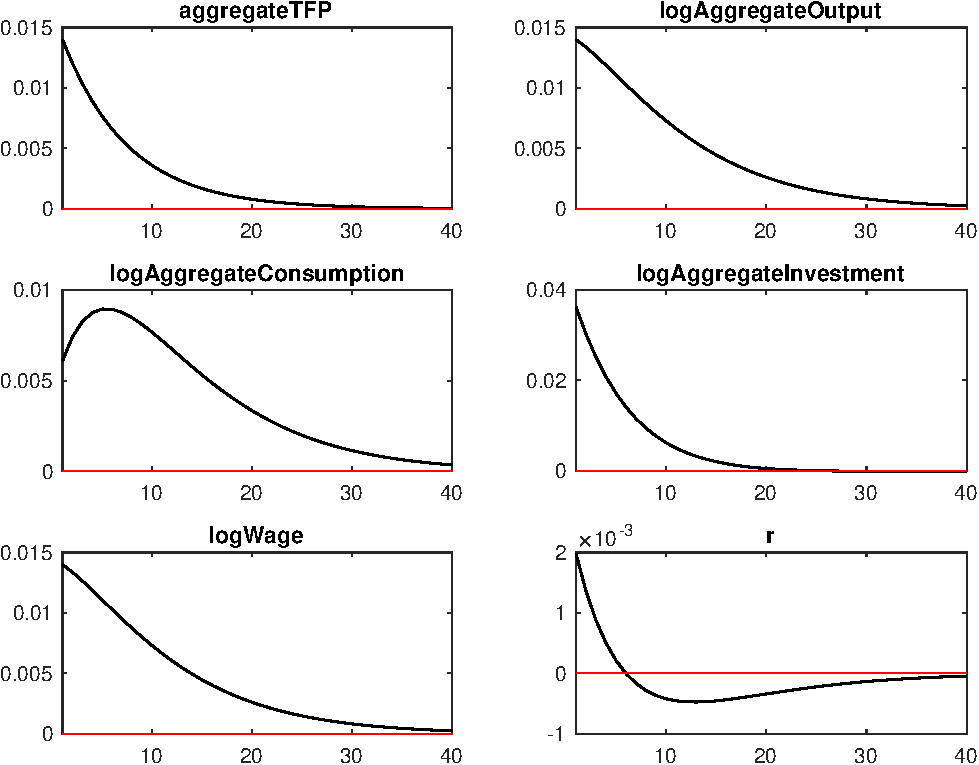
\includegraphics[scale=.355]{./dynamics_polynomials_IRF_aggregateTFPShock_second_order.pdf}
\end{subfigure}
\caption{Replicated impulse response functions around Python computed steady state of Order 1 and Order 2 (from left to right).}
\label{IRF_rep}
\vspace*{\floatsep}
\centering
\includegraphics[scale=.4]{../../../../../../Desktop/Screen Shot 2021-01-25 at 1.25.48 PM}
\caption{Original Figure by Winberry 2018 of order 1 perturbation of Aiyagari model around steady state with respect to TFP}
\label{IRF_orig}
\end{figure*}
\section{Robustness} 
The algorithm's robustness centers on two key assumptions. First, the algorithm will only produce a good approximation to the density if the resulting density is close to the form of a distribution in the exponential family, with some initial mass at 0. If this is not the case, the algorithm will not produce a close fit (though it will produce the projection of the true density onto the exponential family), and may not be useful. Second, if there is a second kink not at some lower bound of the asset space in a policy function, such as from endogenous employment decisions, then the form of the distribution needs to be modified. The most restrictive aspect of the method is that the form of the density and mass points needs to be specified exogenously and in advance. This is a critique that, for example, \cite{Bayer2020} raises with the method. However, it also raises the possibility that the distributional approximation form could be endogenized via a nonparametric method. In particular, a form selected along the lines of sieve MLE or similar nonparametric, but interpolating, procedure might enable a wide number of applications where this method could be both efficient and robust.
\section{Future Extensions}
Future extensions include extending the code to \cite{Winberry2021} fully (it is only partially implemented at the moment, and adding discount rate heterogeneity. Additionally, replacing the parametric estimation of the distribution with a nonparametric technique, whether Sieve MLE or otherwise that captures essential features of the distribution in a low dimensional basis, is a crucial step to extending the technique. Finally, certain aspects of the code can be rewritten in lower level code for performance gains-- the sparse operations which are run 54k times represent an opportunity for speeding up the code dramatically by leveraging some of the C sparse libraries. Additionally areas of the code can be JIT-compiled. \section{Appendix: Algorithm Details} 
\subsection{Young 2010 Implementation}
\code{compute\_MC\_Residual\_Histogram.py} works as follows:
\begin{enumerate}
	\item Solve for the optimal capital level as follows, given an initial guess $K_0$ of capital and $i=0$:
	\begin{enumerate}
	\item Computed implied prices from $K_i$.
	\item Given an initial guess of the next period assets via a rule of thumb decision rule, we loop through and update the EMUC by:
	\begin{enumerate}
	\item On the first iteration only, projecting the current chebyshev polynomial approximation on the next period assets (effectively assuming $E(V'(a',\epsilon'))={a'}^2/2$) and extracting coefficients of  the EMUC-estimating chebyshev polynomial
	\item Using the estimated chebyshev polynomial EMUC to extract next period assets
	\item   Create a new  chebyshev polynomials with zeros on next period assets
	\item Extract an implied future savings and future consumption
	\item  Compute the empirical EMUC $\widetilde{EMUC}$ using estimated future consumption from FOC
	\item  Project the new chebyshev polynomial onto $\widetilde{EMUC}$ to extract new coefficients
	\item  Update coefficients as a mixture between the previous estimate and current estimate and loop back to $(ii)$ until these coefficients converge below a given tolerance level.	
	\item Return an estimate of $EMUC$
	\end{enumerate}
	\item Using the EMUC estimate and FOC, extract implied consumption and savings, as well as endogenous empirical distribution over assets and epsilon $g'(a',\epsilon')$
	\item Aggregate up savings to get a new $\hat{K}_{i+1}$ guess using Gauss-Legendre quadrature (chosen because it performs exact integration for the polynomial integral here.)
	\item Create a true new estimate of $K_{i+1}$ as a weighted sum of $\hat{K}_{i+1}$ and $K_{i}$ 
	\item Check  if $\lVert{K_{i+1} - K_{i}}\rVert_{\infty}<\text{tol} $. If so, return $K_{i+1}\equiv K_{hist}$, else set $i \leftarrow i+1$ and loop back to (a).
	\end{enumerate}
	\item Finally, we run the sequence above one more time up to part c, with the final $K_{hist}$ estimated to extract the implied consumption, savings and distribution of savings (histogram)
\end{enumerate}
\subsection{Parametric Implementation}
\code{compute\_MC\_Residual\_poly.py} works as follows: 
\begin{enumerate}
	
\item Compute the first \code{nmeasure} (here 8) centered moments of the empirical distribution over assets for each $\epsilon$. \code{nmeasure} will represent the truncation order of our parametric exponential family approximation to the distribution.

\item 	Solve for the optimal capital level as follows, given an initial guess $K_{hist}$ of capital and $i=0$:
\begin{enumerate}
\item Computed implied prices from $K_i$.
\item Follow steps (i)-(viii) of \code{compute\_MC\_Residual\_histogram.py} to compute the chebyshev projection of the EMUC
\item Extract the implied asset prime grid using the EMUC estimate
\item Project the exponential family form of the density onto the moments for each epsilon to fit coefficients of exponential family using moment-matching approach
\item Compute new moments and constrained fraction of population using grid over asset space, exponential form and Gauss-Legendre quadrature
\item Compute maximum error between new moments and old moments and new constrained and old constrained fractions. If larger than tol, loop back to (c). 
\item Else, compute $K_{i+1}$ from using $K_{i+1} = $ first moment *  unconstrained fraction + constrained * $\bar{a}$. If $\lVert K_{i+1} - K_{i}\rVert \geq  tol$ then loop back to (a) with $i \leftarrow i+1$.  Else return estimated coefficients of the EMUC, parameters of the exponential family distribution, moments and new capital level. 

\end{enumerate}
\end{enumerate}
\printbibliography
\end{document}


